% %%%%%%%%%%%%%%%%%%%%%%%%%%%%%%%%%%%%%%%%%%%%%%%%%%%%%%%%%%%%%%%%%%%%%%%%%%%%%
\chapter{Non-Autoregressive NMT}
\label{chap:nat}
% %%%%%%%%%%%%%%%%%%%%%%%%%%%%%%%%%%%%%%%%%%%%%%%%%%%%%%%%%%%%%%%%%%%%%%%%%%%%%

The efficiency of \ac{mt} models is often crucial in real-world applications.
Most commercial \ac{nmt} models are available through a cloud-based service,
such as Microsoft Translator\footnote{\url{https://microsoft.com/translator/}}
or Google Translate.\footnote{\url{https://translate.google.com/}} Scaling
cloud-based solutions for large user bases is simple but costly. Even with a
large pool of computational resources, it is worthwhile to implement
optimizations which decrease the model latency and improve the user experience.

Locally-deployed \ac{nmt} models provide a number of advantages over
cloud-based solutions. First, the service does not rely on internet
connection. Second, the data is not being sent to a 3rd party server, and
therefore it is suitable for translating private or confidential data.
However, without optimization, running state-of-the-art translation models
locally often requires specialized hardware, such as one or more GPU
cards. Otherwise, the time for translating a single sentence can easily reach
more than a second on a standard CPU.

Higher decoding speeds can be achieved by model optimization. In their 2019
submission to the \ac{wngt} shared task on efficiency,
\citet{kim-etal-2019-research} successfully employed knowledge distillation,
quantization, shortlisting \citep{jean-etal-2015-using} and a simpler recurrent
unit design to bring the throughput of the translation model up to 3,600 words
per second on a CPU, for a modest drop in the translation quality. Following
this submission, \citet{bogoychev-etal-2020-edinburghs} reported further
improvements with attention head pruning \citep{voita-etal-2019-analyzing}. The
work has been a part of the Bergamot research project, which aims to bring
offline translation models into a browser.\footnote{\url{https://browser.mt/}}

\Ac{nar} models present an alternative approach to model optimization, using a
different architecture and decoding algorithm which has lower time complexity.
In \ac{nmt}, a non-autoregressive decoding algorithm does not access the
previously decoded outputs, imposing conditional independence assumption on the
output token probability distributions. This assumption allows parallelization
of the decoding which can significantly reduce the latency of the translation
system. On the other hand, it also presents a challenge to the language model,
which usually leads to poorer translation quality.

The research presented in this thesis is focused on the usefulness of \ac{nar}
models for translation (\acs{nat}\glsunset{nat}) in the quest for faster
translation models. We first analyze the \ac{nat} models alone and assess the
necessary techniques needed to match the quality of \ac{ar} models.  Then, we
adapt the optimizations successfully used in \ac{ar} models for \ac{nar} models
and evaluate the additional speed gains. \JH{This is currently not in the
  thesis. We'll have shortlisting with a fast implementation.}

In this chapter, we present an overview of the current state of the research
and the key concepts in non-autoregressive \ac{nmt}. We begin with the
description of the principles that most of the literature on this topic has in
common in Section \ref{sec:nat:principles}. Then, we provide a survey of
notable approaches to \ac{nat}. We categorize the studied methods into four
groups, each of which is described in separate section. The methods most
similar to our work are based on a relaxed alignment between the output and
target sequences (Section \ref{sec:nat:alignment}). Methods that improve the
training process using auxiliary objectives are described in Section
\ref{sec:nat:aux}. Section \ref{sec:nat:semi} introduce approaches based on
iterative decoding. Natually, the groups are not mutually exclusive and there
is an overlap. Relevant methods not falling clearly into any of the categories
above are summarized in Section \ref{sec:nat:misc}.  We conclude this chapter
with a discussion of the limitations of the presented literature, mostly
concerning the evaluation methodology.


% ------------------------------------------------------------------------------
\section{Non-Autoregressive Models}%
\label{sec:nat:principles}
% ------------------------------------------------------------------------------

This section summarizes the main features of \ac{nar} models and some of the
basic concepts and the research problems in this field. The \ac{nar} variant of
the Transformer model was first described by \citet{gu2017nonautoregressive}
and \citet{lee-etal-2018-deterministic}. Each of these two foundational papers
provides different (complementary) grounds for further research discussed later
in this chapter -- using latent variables, and iterative decoding.

% ------------------------------------------------------------------------------
\paragraph{Conditional Independence.} The defining feature of a
non-autoregressive model is the assumption of conditional independence between
the output distributions across time steps. Recall Equation
\ref{eq:output-distribution} which defines the output distribution for
autoregressive models:
%
\begin{equation*}
  p(y|x) = \prod_{t=1}^{T_y}p(y_t|y_{<t},x,\theta).
  \tag{\ref{eq:output-distribution}}
\end{equation*}
%
Unlike Equation \ref{eq:output-distribution}, \Ac{nat} models do not condition
the output token probabilities on the previously decoded outputs $y_{<t}$.  The
probability of an output sentence $y$ given an input sequence $x$ can then be
modeled as:
%
\begin{equation}
  p(y|x) = \prod_{t=1}^{T_y}p(y_t|x,\theta).
  \label{eq:nat-output-distribution}
\end{equation}

Although technically possible, making the outputs in \acs{rnn}-based models
conditionally independent does not reduce the time complexity because in
\acsp{rnn}, the value of each hidden state depends on the value of the
preceding state. However, in the Transformer model, hidden states in one layer
depend only on the states from the previous layer. This allows for
parallelization of the computation on the layer level.

Since the outputs are conditionally independent, we cannot feed the previously
decoded outputs into the Transformer decoder. In the following paragraphs, we
discuss the necessary alterations to the Transformer architecture. We need to
provide the decoder inputs and estimate the target length. The causal mask in
the decoder self-attention is now unnecessary. We also address the main issue
and the reason \ac{ar} models are still superior in modeling language.

% ------------------------------------------------------------------------------
\paragraph{Multimodality Problem.} In one of the first applications of a
non-autoregressive model to \ac{nmt}, \citet{gu2017nonautoregressive} describe
the \emph{multimodality problem} which arise when the outputs are conditionally
independent.

When estimating the probability of a word on a given position, there may be
multiple words which get a high probability. These words are the so called
\emph{modes} of the distribution. In autoregressive models, once a word gets
selected, other modes are ignored in the following time steps. However, a
non-autoregressive model does not base the decisions on the preceding ones, so
when multiple positions have multiple modes, the model has no means to
coordinate the selection of modes across different time steps.

% This issue is illustrated in Figure \ref{fig:multimodality-problem}.
% \begin{figure}
%   \centering
%   \begin{minipage}{\textwidth}
%     source: thank you

%     \begin{center}
%     \begin{tabular}{cccc}
%       \toprule
%       $y_1$ & $p(y_1|x)$ & $y_2$ & $p(y_2|x)$ \\
%       \midrule
%       vielen & 0.4 & dank & 0.4 \\
%       danke  & 0.3 & schön & 0.3 \\
%       \vdots & & \vdots & & \\
%       \bottomrule
%     \end{tabular}
%     \end{center}

%   \end{minipage}
%   \caption{Illustration of the multimodality problem.}
%   \label{fig:multimodality-problem}
% \end{figure}

A well-known example of the multimodality problem is the translation of the
sentence ``thank you'' into German, which has two equally likely translations:
``vielen dank'' and ``danke schön.'' In this case, the pair of German tokens
``danke'' and ``vielen'' create the two modes on the first position, and the
tokens ``dank'' and ``schön'' are the modes on the second position. If an
\acl{ar} model chooses to generate ``danke'' on the first position, the token
``dank'' on the second position will no longer receive high probability by the
model. However, when a \acl{nar} model assigns high probabilities to the
correct translations, it also has to assign high probabilities to the other
(incorrect) two combinations, ``danke dank'' and ``vielen schön''. \JH{Come up
  with a different example.}

% ------------------------------------------------------------------------------
\paragraph{Target Length Estimation.} In a standard NMT model such as the
Transformer or an \acs{rnn}-based model with attention, the length of the
output sentence is modeled implicitly by using the special end-of-sentence
(\eos{}) token. Equations \ref{eq:output-distribution} and
\ref{eq:nat-output-distribution} work with the sentence length implicitly,
assuming that the last token $y_{T_y}$ is the \eos{} token and that \eos{} does
not appear among the previous tokens $y_{<T_y}$.

The probability distribution in Equation \ref{eq:nat-output-distribution} can
be factorized to express the estimation of the target sentence length
explicitly: %leaving out the \eos{} symbol from the mathematical model:
\begin{equation}
  p(y|x, \theta) = p_L(T_y|x, \theta) \cdot \prod_{t=1}^{T_y}p(y_t|x,\theta).
  \label{eq:explicit-length}
\end{equation}

The explicit target length estimation is a useful technique of moderating the
multimodality problem. It also helps with the problem of supplying the inputs
for the decoder, as seen in many of the approaches described here.

% ------------------------------------------------------------------------------
\paragraph{\Ac{nat} with Fertility Model.} \Acs{nar} Transformer decoder cannot
receive the previously decoded tokens on the input. A solution proposed by
\citet{gu2017nonautoregressive} is to use a simple fertility model, which also
serves as the explicit target length estimator.

Compared to the autoregressive Transformer model, the model has the following
modifications. First, the inputs to the decoder are made up of the sequence of
encoder inputs, either uniformly stretched to the predicted target sentence
length, or copied using a fertility model. Second, the decoder self-attention
does not use the causal mask since all states can now attend to all other
states in both directions. Third, \emph{positional attention} is added to every
decoder layer where the positional encoding is used as queries and keys, and
the decoder states as values.

In \citet{gu2017nonautoregressive}, the multimodality problem (and the length
estimation) is addressed by introducing a latent fertility variables
$F = f_1, \ldots, f_{T_x}$ sampled from a prior distribution. Each
$f_i \in \mathbb{N}_0$ denotes the number of times to copy $x_i$ to the decoder
input (summing up to the target length $T_y$). The output probability is then
conditioned on the latent variable $F$, which is marginalized out:
%
\begin{equation}
  p(y|x, \theta) = \sum_{F \in \mathcal{F}} p(F|x, \theta) \cdot p(y|x, F, \theta)
\end{equation}
%
where the fertility model $p(F|x, \theta)$ and the translation model
$p(y|x, F, \theta)$ can be trained jointly using a variational lower bound with
a candidate distribution $q$:
\begin{align}
  \begin{split}
    \mathcal{L}(\theta)
    & = \log p(y|x, \theta) = \log \sum_{F \in \mathcal{F}} p(F| x, \theta ) \cdot p(y | x, F, \theta) \\
    & \geq \mathbb{E}_{F \sim q} \left(\sum_{t=1}^{T_y} \log p(y_t | x, F, \theta)
      + \sum_{t=1}^{T_x} \log p(f_t | x, \theta) \right) + \mathcal{H}(q)
  \end{split}
\end{align}
%
where $q$ is an external deterministic fertility model, and therefore
$\mathcal{H}$ is a constant and the expectation is also deterministic. \JH{I
  dont completely understand but assume that there is a single sample with
  probability of 1, so you just minimize the inside of the big bracket and
  ignore the rest.}
%
The fertility model depends on an external module which is not trained together
with the model. The authors fine-tune the trained model using reinforcement
learning \citep{williams1992simple}.

During decoding, the marginalizing over all possible fertility values is
intractable. Therefore, the authors experiment with three approximation methods
-- argmax and average decoding, and \ac{npd}.

% ------------------------------------------------------------------------------
\paragraph{Autoregressive Rescoring.} A usual technique in the \ac{nat}
literature is to use some form of rescoring of the outputs of the \acl{nar}
model by an \acl{ar} model. The nature of the Transformer model allows to score
a sentence in a single step (as opposed to generating one), which means that
the additional rescoring computation increases the decoding complexity only
linearly with respect to the number of the candidate hypoteheses for rescoring.

The choice of the rescoring candidates varies. \citet{gu2017nonautoregressive}
use \ac{npd} which first samples the decoder input sequences from the fertility
distribution, compute the best candidate for each input, and then rescore the
results using the \ac{ar} teacher model. A closely related method is \ac{lpd}
which generates and scores sentences of different lengths.

Note that in contrast to \ac{ar} models, the highest-scoring sequence in an
\acs{nar} model can be found simply by taking the highest-scoring token in each
step, because of the conditional independence assumption.

% ------------------------------------------------------------------------------
\paragraph{Knowledge Distillation.} To tackle the multimodality problem from
another angle, \citet{gu2017nonautoregressive} propose to use sequence-level
knowledge distillation to create artificial training data
\citep{kim-rush-2016-sequence}. The main idea is that outputs of a teacher
model will have a simpler structure than natural language, limiting the number
of the distribution modes.

According to an ablation study published by \citet{gu-kong-2021-fully}, using
knowledge distillation is a crucial element in training non-autoregressive
translation models, regardless the actual method used.
\citet{zhou-etal-2020-understanding} further study the effects of knowledge
distillation strategies on the translation quality of \ac{nar} models.

% ------------------------------------------------------------------------------
\paragraph{Iterative Refinement.} Another attempt to introduce latent variables
in a \acl{nar} model was proposed by \citet{lee-etal-2018-deterministic}.
Instead of modeling fertility, the authors introduce $L$ discrete sequential
latent variables interpreted as stages of refinement:
%
\begin{align}
  \begin{split}
    p(y|x) & = \sum_{y^L}
      \left( \prod_{t=1}^{T_y} p(y_t|y^L, x) \right) p(y^L|x) \\
    p(y^L|x) & = \sum_{y^{L-1}}
      \left( \prod_{t=1}^{T_y} p(y_t^L | y^{L-1}, x) \right)
      p(y^{L-1}|x) \\
    \vdots \\
    p(y^0|x) & = \prod_{t=1}^{T_y} p(y_t^0|x)
  \end{split}
\end{align}
%
Each summation in the equations above is computed over the whole space of
possible sequences, and thus, it is intractable for the probablility $p(y|x)$
to be caluculated exactly. To overcome this problem, the authors approximate
the sums with only the element corresponding to the sequence with the largest
probability, $\hat{y} = \argmax_{y}p(y|x)$.% \footnote{Note that in
  % non-autoregressive model where the probability does not depend on previously
  % decoded outputs $y_{<t}$, getting the most probable tokens will also yield
  % the most probable sequence.}
Putting it together with the equations above
and moving to the logarithmic domain, we get:
\begin{align}
  \begin{split}
    \log p(y|x) \geq
    & \sum_{t=1}^{T_y} \log p(y_t| \hat{y}^L, x) + \\
    & + \sum_{t=1}^{T_y} \log p(\hat{y}_t^{L}| \hat{y}^{L-1}, x) + \ldots \\
    & + \sum_{t=1}^{T_y} \log p(\hat{y}_t^0 | x). \label{eq:refinement-lowerbound}
    % = & \sum_{l=0}^{L} \sum_{t=1}^{T_Y} \log p(\hat{y}_t^{l+1} | \hat{Y}^l, X)
  \end{split}
\end{align}
%where $Y^0 = X$ and $\hat{y}_t^{L+1} = y_t$.

The tokens $\hat{y}_t^0$ in the initial sequence are set to $x_{t'}$ where
$t' = (T_x / T_y) \cdot t$, i.e. the source sentence is either squished or
stretched by copying or omitting some of the source words in order to fit the
target sentence length. During training, the length of the reference sentence
is known. During decoding, the authors use a separate model $p(T_y|x)$ for
target length prediction. All probability distributions in the above equations
are modeled with neural networks with shared parameters. In this way, the
number of intermediate refinement steps remains flexible during the decoding.

The latent variable model is trained by minimizing the log-likelihood of the
reference sentence $y^*$ in each of the refinement steps:
\begin{equation}
  \mathcal{L}_{\text{LVM}}(\theta) = - \sum_{l=1}^{L+1} \left(
    \sum_{t=1}^{T_{y^*}} \log p(y_t^* | \hat{y}^{l-1}, x, \theta)
  \right) \label{eq:refinement-lvm-loss}
\end{equation}

In their iterative approach, \citet{lee-etal-2018-deterministic} also discuss
the training of the refinement process from a denoising perspective. Formally,
they introduce an additional denoising autoencoder loss to the model:
%
\begin{equation}
  \mathcal{L}_{\text{DAE}}(\theta) = - \sum_{t=1}^{T_y} \log p(y_t^* | \bar{y}, x, \theta)
\end{equation}
where $\bar{y}$ is a corrupted version of the reference translation $y^*$. The
corruption process is performed on each token with a probability $\beta$. Each
corrupted token is either replaced with a random word from the vocabulary,
copied to its neighbor, or swapped with the neighbor.

During training, the two loss functions are stochastically mixed using a
hyperparameter $\alpha$, sampled from a Bernoulli distribution.


% ------------------------------------------------------------------------------
\section{Alignment-Based Methods}%
\label{sec:nat:alignment}
% ------------------------------------------------------------------------------

\Acl{ar} models are trained using the cross-entropy loss (recall Equation
\ref{eq:loss}). When we assume a single sentence pair $(x,y)$, the negative
log-likelihood is the sum of negative log-probabilities
$\log p(y_i|x, y_{<i}, \theta)$ for $i=1, \ldots, T_y$, as estimated by the
model with parameters $\theta$.  Notice how the ground-truth sequence
$y_1, \ldots, y_{T_y}$ corresponds to the sequence of the probabilities
$p(y_i|\ldots)$: we require that the $i$-th reference token is decoded at the
$i$-th position of the output state sequence. The methods described in this
section relax this requirement.

We define an alignment as a function $a$ which maps the positions in the
ground-truth sentence to the positions in the output. In autoregressive
models, $a(i) = i$ for every position $i$ in the ground truth. % When we
% generalize the cross-entropy loss for sentence pair $(x, y)$ to account for the
% alignment, we get
Methods that consider different alignments allow to work with output and label
sequences with different lengths, which is a useful feature in the context of
\ac{nat} models.

To the best of our knowledge, we were the first to propose an alignment-based
method for \ac{nat} \citep{libovicky-helcl-2018-end}. Our method is based on
\acf{ctc}\glsunset{ctc}, which computes the cross-entropy losses over all
possible alignments between the ground truth and a longer output state
seqeunce. We describe this method in detail in Chapter \ref{chap:nar-nmt-ctc}.
In the following paragraphs, we present a number of related methods based on
modeling the alignment between the sequences of outputs and ground-truth
labels.

% -----------------------------------------------------------------------------
\paragraph{Aligned Cross Entropy for \ac{nat}} One problem with using
cross-entropy objective for training \ac{nat} models is that it heavily
penalizes misaligned target words. If a correct word is generated at an
incorrect position in the target sentence, it does not have a positive effect
on the loss, same as when a completely unrelated word is generated. In \acl{ar}
models, this problem is avoided with teacher forcing -- the model is provided
with the preceding words from the reference sentence. Without teacher forcing,
the alignment between the predicted distributions and the positions in the
reference sentence is too rigid. For example, consider the reference sentence
``Thank you for your cooperation.'' In a \acl{nar} model, another translation
``Thanks for your cooperation'' receives the same training signal as a
completely wrong translation. The difference is that on the second position,
the autoregressive model knows that ``Thank'' was expected on the first
position, so the next word ``for'' does not receive high probability.  One way
to address this problem is to consider the alignment as a latent variable.

\Acl{axe} \glsunset{axe} (\acs{axe}; \citealp{ghazvininejad2020aligned}) is an
objective function that takes this problem into account. It uses a dynamic
programming algorithm to find the alignment with the minimum cross-entropy
loss. In the example from the previous paragraph, the alignment with the lowest
cross-entropy is the one that aligns the positions 3--5 from the label sequence
(representing the suffix ``for your cooperation'') to output positions 2--4 in
the output. Either of the first two positions in the label sequence can be
aligned to the first position in the output sequence, while the other label
position remains unaligned.

The alignments considered in the \ac{axe} approach are monotonic (i.e.
$a(i) \leq a(j)$ for every $i \leq j$, when defined), but the mapping does not
have to be defined for each ground-truth position, as well as any position in
the prediciton sequence is not required to be mapped to a reference position.
In case of skipping a prediction, the model learns to output an empty token
$\epsilon$ ($-\log p(y_t = \epsilon | x, \theta)$ is added to the loss).  When
a position in the ground-truth sequence is skipped, the negative
log-probability of the skipped token is added to the loss at the current
prediction position, weighted by a hyperparameter $\delta$ which controls the
cost of the skip-target operation.  The alignment with the minimum
cross-entropy is chosen for computing the gradients and updating the model.

The authors use \aclp{cmlm} as the base architecutre (described later in
Section \ref{sec:nat:semi}).  Since the empty tokens are discarded during
decoding, the authors choose similar approach to
\citet{libovicky-helcl-2018-end} and initialize the decoder input length with
the source length multiplied by a factor of $\lambda$, which they estimate
empirically from the dataset.

In our experiments, we use the \ac{ctc} loss, which is similar to this
approach. Instead of considering the alignment that yields the minimum
cross-entropy loss, the \ac{ctc} algorithm computes the sum of all the possible
alignments. Unlike \ac{axe}, we only consider skipping the predictions, while
not allowing to skip the target positions. We present the \ac{ctc}-based method
in detail in Chapter \ref{chap:nar-nmt-ctc}.

% -----------------------------------------------------------------------------
\paragraph{Order-Agnostic Cross-Entropy.} The alignment-based method discussed
in the previous paragraphs considers only monotonic
alignments. \citet{du2021orderagnostic} design \ac{oaxe}, a new training
objective which also permits non-monotonic alignments (see illustration in
Figure \ref{fig:oaxe-example}). Similarly to \ac{axe}, they select the ordering
with minimum cross-entropy for gradient propagation.

\begin{figure}
  \centering
  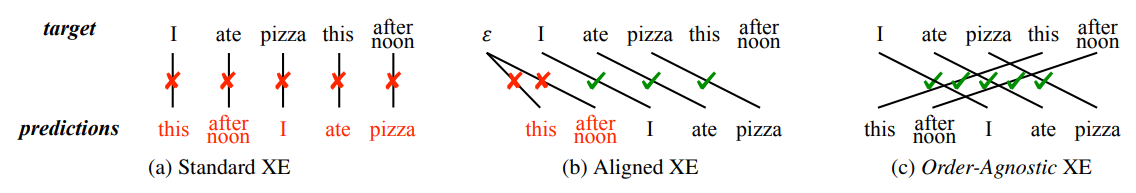
\includegraphics[width=\textwidth]{img/oaxe.png}

  \caption{An illustration of (a) cross-entropy, (b) aligned cross-entropy, and
    (c) order-agnostic cross-entropy on a toy example. We use the figure from
    \citet{du2021orderagnostic}, Figure 1}%
  \label{fig:oaxe-example}
\end{figure}

The dynamic programming algorithm used in the \ac{ctc} and \ac{axe} methods is
no longer suitable for non-monotonic alignments. Moreover, the search space is
even larger than in the previous case as it is proportional to the factorial of
the target length. The authors use the Hungarian algorithm
\citep{kuhn1955hungarian} which finds a maximum bipartite matching in a
polynomial time. They also incorporate heuristics and tweak the search
algorithm to exclude invalid orderings or predictions.

% ----------------------------------------------------------------------------
\paragraph{Imputer.} Antoher variant of the alignment-based approach was
described by \citet{saharia-etal-2020-non}. In the paper, they experiment with
a \acs{ctc}-based model similar to the model we use in this thesis, and an
iterative variant called \emph{Imputer}.

The model architecture is a stack of self-attentive layers without the causal
mask. The \acs{ctc}-based model takes upsampled source sentence embeddings (in
order to be able to create translations which are longer than the source) and
processes them with the Transformer layer stack.  The Imputer model proceeds in
a fixed number $L$ of iterations. In each iteration, the model generates
(``imputes'') $\ceil*{\frac{T_y}{L}}$ on some positions where $T_y$ is the
output length. This procedure is similar to decoding from \aclp{mlm} described
in Section \ref{sec:nat:semi}. Additionally to the \ac{ctc} model, the input to
the Imputer model is the embedding of the partially decoded sentence from the
previous iteration summed with the (upsampled) source sentence embeddings.

The training of the Imputer model takes into account every partial output
potentially already decoded and maximizes a log-likelihood lower bound, which
can be comptued with a dynamic programming algorithm. \JH{more needed? or
  less?}


% ------------------------------------------------------------------------------
\section{Auxiliary Objective Methods}%
\label{sec:nat:aux}
% ------------------------------------------------------------------------------

Auxiliary objectives can be viewed as a form of regularization of the training
process. Unlike techniques that aim at improving the convergence speed, such as
$L_2$ regularization or dropout, the objectives described here are designed to
help \acl{nar} models cope with the conditional independence assumption in
order to better model the target language.

The following methods are based on including one or more auxiliary objectives
into the training procedure. Unlike the methods in different sections which
also use auxiliary objectives, none of these methods changes the decoding
process, which is done by taking the highest-scoring token in each time step in
parallel.

% ------------------------------------------------------------------------------
\paragraph{\Ac{nat} with Auxiliary Regularization.}
\citet{wang-etal-2019-nonautoregressive} analyze the basic \ac{nat} model
\citep{gu2017nonautoregressive} and identify two frequent translation errors --
repeated and incomplete translation. For each of these symptoms, they design a
special auxiliary objective to mitigate their effect.

For the repeated translation problem, where the same token is generated
multiple times in conseutive time steps, the authors propose to increase the
dissimilarity of adjacent hidden states when different tokens should be
decoded, tiyng the similarity of the target token embeddings to the similarity
of the corresponding hidden states.

The incomplete translation problem is a case of tokens missed out from the
translation. To battle this problem, an reverse \ac{ar} translation model is
used to reconstruct the source sentence back from the decoder output states.
The loss of this backward translation model is again used as an auxiliary
objective.

In the final \acs{natreg} model, the two auxiliary losses are mixed in with the
standard cross-entropy loss, using weight hyperparameters which are set
empirically.

% ------------------------------------------------------------------------------
\paragraph{\Acs{hintnat}.} As mentioned in the introductory section of this
chapter, knowledge distillation is used quite often in \ac{nat}
research. \citet{li-etal-2019-hint} decide to use the \ac{ar} teacher model to
provide signals (hints) to the training of the student model.

They propose to use two types of hints from the teacher model. First, to bring
the values of the decoder hidden states closer together the authors consider
tying the teacher and student states with $L_1$ or $L_2$ distance, but argue
that this straightforward approach destabilizes the student training process
and fails. Instead, they use a weaker signal from the teacher model and define
an auxiliary loss based on the cosine distances within the decoder hidden
states. Second, they use the information from the teacher model cross-attention
to guide the alignment learning in the student model. Again, this information
is incorporated into the training as an auxiliary loss, based on the KL
divergence between the teacher and student attention distributions.  Again, the
auxiliary losses are mixed using weighting hyperparameters along with
the cross-entropy loss.

% -----------------------------------------------------------------------------
\paragraph{\Acl{bon} Difference.} \citet{shao2020minimizing} address the
issue of misalignment between the targets and the outputs. Instead of finding
an appropriate alignment, they design a new \acf{bon}\glsunset{bon} objective,
which minimizes the difference between the \ac{nat} model output and the target
sentence.

The \ac{bon} objective is based on the $L_1$ distance between two sparse
vectors representing the n-grams which are present in the reference sentence
and are likely to be present in the translation (based on the output
probabilities). As in the previous two cases, this objective is complemented by
the cross-entropy objective. The authors also show that fine-tuning with the
\ac{bon} objective alone is helpful.

% -----------------------------------------------------------------------------
\paragraph{Glancing Training.} \citet{qian-etal-2021-glancing} propose
\acf{glat}\glsunset{glat}, a technique for training the \ac{nat} model
similarly to \acp{cmlm}, but enabling decoding in a single pass instead of an
iterative process.

During training, the model first generates an intermediate output sentence
non-autoregressively. Then, a number of positions is masked according to a
glancing sampling strategy, and the model is trained to predict the masked
tokens on the selected positions. The sampling strategy randomly selects $S$
positions, where $S$ is proportional to the number of errors in the
intermediate prediction.

The decoding is similar to the process proposed by
\citet{gu2017nonautoregressive}, but instead of the fertility model, the target
length prediction is done using an artificial token \texttt{LENGTH} and its
representation to predict the target length (as in the \ac{cmlm} approach of
\citealp{ghazvininejad-etal-2019-mask})

Very recently, a \ac{glat} model appeared among the top-scoring models at the
\acs{wmt} news translation shared task \citep{qian2021volctrans}. \JH{update
  bib after WMT}


% ------------------------------------------------------------------------------
\section{Iterative and Semi-Autoregressive Methods}%
\label{sec:nat:semi}
% ------------------------------------------------------------------------------

The common theme in all of the approaches described so far is that during
inference, the underlying Transformer model is executed only once.  \Acl{ar}
models, on the other hand, need $T_y$ executions to generate a sentence of
$T_y$ tokens. This linear relationship follows from the conditional dependency.

In this section, we look at methods that lie somewhere in between. In these
approaches, the number of model executions is greater than one, but it is still
constant with respect to the target length $T_y$. We call these approaches
\emph{iterative}. We also include approaches which operate in a fraction of
$T_y$ steps, even though the number of steps is no longer constant. We refer to
these approaches as \emph{semi-autoregressive}.

Many of the methods described here are based on the ideas of iterative
refinement first introduced by \citet{lee-etal-2018-deterministic}, which we
have already reviewed in the introductory section.

% ------------------------------------------------------------------------------
\paragraph{Iterative Decoding from Masked Language Models.} Recently,
pre-trained \acp{mlm} such as BERT \citep{devlin-etal-2019-bert} have attracted
attention from the translation research
community. \citet{ghazvininejad-etal-2019-mask} introduce
\acfp{cmlm}\glsunset{cmlm}, an extension to \acp{xlm} for multilingual
applications, including \ac{mt} \citep{conneau-lample-2019-cross}.

Conventional \acp{lm} estimate the probability of a word given the preceding
words.  In contrast, \acp{mlm} are trained on sentences where a number of
tokens has been masked-out, and the objective is to predict what the masked
words were, given the rest of the sentence. \Acp{xlm} extend this idea to a
pair of sentences in two (or more) languages. That is, tokens from either
source, or target sentence, or both, are masked and the model tries to predict
them.  To facilitate for alignment modeling and language identification,
\ac{xlm} architectures include a language embedding and reset the positional
encodings for each sentence. See Figure \ref{fig:mlm-xlm-example} for an
illustration of the difference between \acp{mlm} and \acp{xlm}.

\begin{figure}
  \centering

  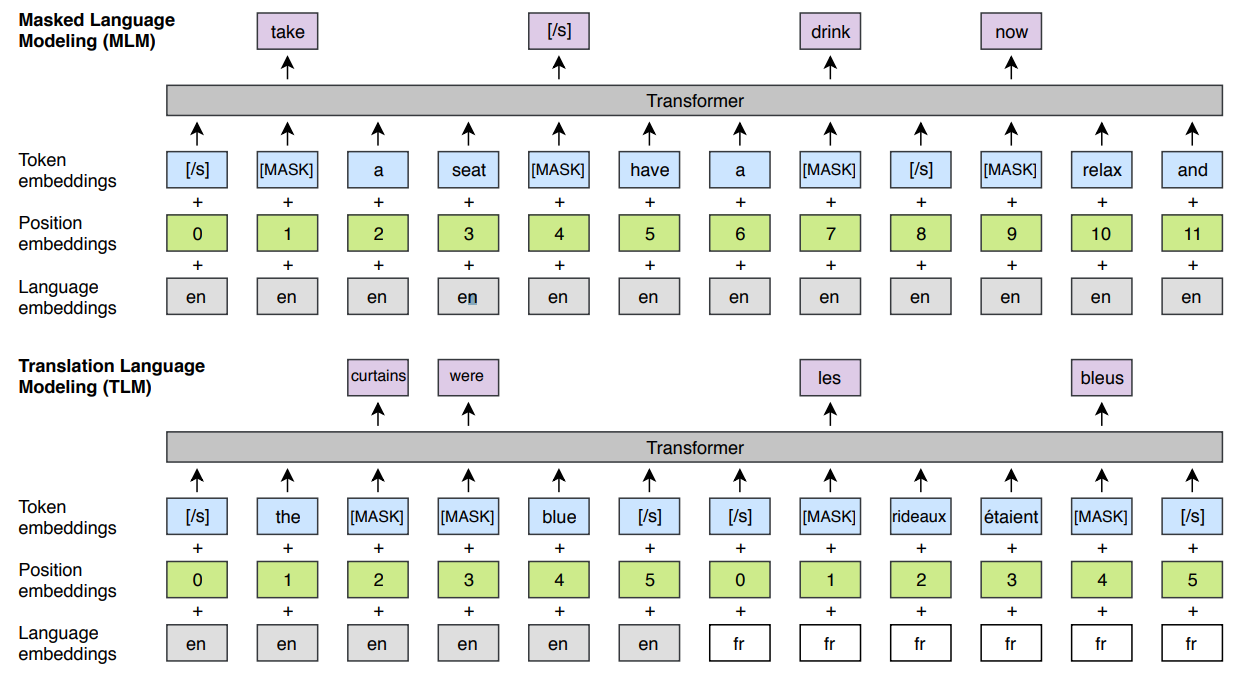
\includegraphics[width=\textwidth]{img/mlm-xlm.png}

  \caption{A comparison of masked language model and translation
    (cross-lingual) language model architectures. We use the image of
    \citet{conneau-lample-2019-cross}, Figure 1.}%
  \label{fig:mlm-xlm-example}
\end{figure}

\Aclp{cmlm} originate in the ideas of
\citet{conneau-lample-2019-cross}. However, there are a few differences. First,
\acp{cmlm} use an encoder-decoder architecture, rather than a decoder-only
model that works on the concatenation of the source and target
sentences. Second, only the target words are masked and subject to the training
and prediction. \Acp{cmlm} are also intended for use in the end-task, rather
than for cross-lingual \ac{lm} pretraining, as is the case of \acp{xlm}.

The decoding process starts with the estimation of the target length. For this
purpose, \citet{ghazvininejad-etal-2019-mask} include a special \texttt{LENGTH}
token in the decoder input and predict the target length as the output on this
position. This way the length predictor can be trained jointly with the
translation model using the cross entropy training signal. The authors show
that it is useful to sample a small number of different length candidates,
decode a translation for each length, and then pick the highest scoring one.

Given a target length, the generation begins with a sequence of mask symbols.
In each iteration, the tokens on all masked positions are predicted in parallel
(independently, and thus, non-autoregressively). Then, a number of the tokens
that receive the lowest probability by the model is selected and masked-out
again, prepared to be re-predicted in the next iteration. The number of the
masked tokens is decreasing with each iteration, so that a constant number of
iterations is needed to generate the whole translation.

In their generalized framework for sequence generation,
\citet{mansimov2019generalized} experiment with other masking strategies, such
as left-to-right, easy-first, or uniform.

% ------------------------------------------------------------------------------
\paragraph{SMART.} In their follow-up experiments,
\citet{ghazvininejad-etal-2020-semiautoregressive} address the exposure bias
issue in context of \acp{cmlm} (although they use the terms autoregressive and
non-autoregressive for the distinction between using the model predictions
during training and teacher forcing).

As discussed in Section \ref{sec:training}, the exposure bias problem arises
when the model is trained on ground-truth data, but during decoding, it relies
on its own (often incorrect) decisions instead. \Acp{cmlm} are trained to
predict masked tokens given the ground-truth context, but during decoding, the
refinement is done using generated context instead.

To tackle this issue, \citet{ghazvininejad-etal-2020-semiautoregressive}
propose to mix the ground-truth tokens with the model predictions. This
approach is somewhat similar to scheduled sampling for \aclp{rnn}
\citep{bengio2015scheduled}.

% ------------------------------------------------------------------------------
\paragraph{DisCO.} %\textbf{iterative, change to the attention and objective}
\citet{kasai2020nonautoregressive} extend the \ac{cmlm} model with a few
additions. Instead of predicting only the masked tokens, the authors propose an
architecture that is able to predict a subset of the \emph{other} tokens for
each position in the target sequence. They achieve this goal by adapting the
attention module. First the self-attention does not attend to the same position
in the previous layer. Second, to prevent information leakage between the same
positions on different layers, the self-attention keys and values are
decontextualized, meaning that instead of the hidden states from the previous
layer, the decoder input embeddings are used.

% ------------------------------------------------------------------------------
\paragraph{JM-NAT} %\textbf{iterative, auxiliary objective}
Following the practice from training the BERT model
\citep{devlin-etal-2019-bert}, \citet{guo-etal-2020-jointly} mask source words
in the encoder in each step to achieve a more robust encoder
representation. They introduce an auxiliary loss in the encoder, for predicting
the masked tokens.

Instead of masking out random tokens in the decoder, the authors propose to
mask whole random n-grams. They also use another auxiliary n-gram loss tailored
to help with the problem of repetitive tokens in the translation. The
mask-predict strategy \citep{ghazvininejad-etal-2019-mask} is employed during
inference.

% ------------------------------------------------------------------------------
\paragraph{Semi-Autoregressive \acs{nmt}} One of the first attempts to bring
together the best of the worlds of \ac{ar} and \ac{nar} models was proposed by
\citet{wang-etal-2018-semi}. In their work, the authors use a
semi-autoregressive Transformer model which predicts groups of $K$ consecutive
tokens at a time. The tokens in each group are predicted independently and in
parallel, but the conditional dependency is retained between the groups in
autoregressive fashion.

As expected, the authors find that increasing $K$ leads to degraded translation
quality, but brings improvements in terms of decoding speed.

% ------------------------------------------------------------------------------
\paragraph{Blockwise Parallel Decoding for Deep Autoregressive Models.}
\citet{stern2018blockwise} propose a similar semi-autoregressive approach where
chunks of the target sentence are generated in parallel.
%
They start with a greedy decoding from an autoregressive model, $p_1$, and
introduce additional ``look-ahead'' models $p_2, \ldots p_k$. In time step $t$,
each model $p_i$ predicts the $(t + i)$-th word in the target sequence given the
same prefix of $t$ previously decoded words.

The decoding process has three stages. First, the block of predictions using the
models $p_1, \ldots, p_k$ is computed. Second, model $p_1$ is used to verify the
$(k-1)$ candidates (which is done in parallel in the Transformer model) and
finds the largest $\hat{k}$ such that decoded words from models $p_i$,
$1 \leq i \leq \hat{k}$ are all considered best by $p_1$. Third, the accepted
$\hat{k}$ words are generated and the decoding process jumps to time step
$t + \hat{k}$.

% ------------------------------------------------------------------------------
\paragraph{Insertion Transformer.} The Insertion Transformer
\citep{stern-etal-2019-insertion} is an extension of the Transformer model
which handles sequence generation in an arbitrary order. Instead of predicting
tokens left-to-right, the model predicts sequences of insertion operations. An
insertion operation specifies what tokens to insert, and where to insert
them. In each step, the insertion operations are generated in parallel and
independently. Thus, we can include this approach in the semi-autoregressive
category. The authors experiment with decoding in a balanced binary-tree order,
which can generate the output sequence in a logarithmic number of steps.

% An extension to the Insertion Transformer is
% KERMIT. \citep{chan-etal-2019-kermit} \JH{more about kermit}

% ------------------------------------------------------------------------------
\paragraph{Levenshtein Transformer.} An interesting combination of the ideas
introduced in Insertion Transformer and \acp{cmlm} is the \acl{levt}
(\acs{levt}\glsunset{levt}; \citealp{gu-etal-2019-levenshtein}). This model
operates in an iterative fashion, much like the aforementioned methods. At the
beginning, \ac{levt} takes either an empty sentence or a crude, intermediate
sentence for refinement. Each iteration consists of applying three
policies. First, tokens to be deleted are identified and removed from the
sequence. Second, each slot (a position between two tokens) is assigned with a
number, and this number of placeholder symbols is inserted into the slot.
Third, for each placeholder, a token from the vocabulary is selected and the
placeholder symbols are replaced with the selected tokens, resulting in a
refined version of the input sentence.  Each of the three stages of a
refinement iteration is performed non-autoregressively.

% ------------------------------------------------------------------------------
\paragraph{Latent Transformer.} \citet{kaiser2018fast} use discrete latent
variables in a model called \acf{lt}\glsunset{lt}. The model has three
components. First, the \emph{autoencoder} takes a sentence pair $(x, y)$ and
encode the target sentence $y$ into a sequence of discrete latent variables
$l$. Second, an \acl{ar} \emph{latent prediction} model, which predicts the
sequence $l$ based on a source sentence $x$. Third, an \acl{nar}
\emph{decoder}, used to generate $y$ given the source sentence $x$ and the
hidden sequence $l$.

The autoencoder is used for training in order to condense the longer target
sequence $y$ into a shorter (usually 8 times) sequence $l$, which is used as an
itermediate representation of $y$. Unlike perhaps more common autoencoders,
this autoencoder uses discrete latent variables. The authors propose two
methods (decomposed vector quantization and latent semantic hashing) for the
discretization. A stack of convolutions with residual connections is selected
as the autoencoder architecture. The latent predictor is a stack of Transformer
layers, and the decoder consists of up-convolutions.


% ------------------------------------------------------------------------------
\section{Other Methods}%
\label{sec:nat:misc}
% ------------------------------------------------------------------------------

In this section, we summarize the related work that does not fall clearly
within any of the three categories from the sections above.

% \paragraph{LaNMT} \citep{shu2020latent} -- latent-variable NAR NMT with
% deterministic inference using a delta posterior \JH{to bych nechal na potom
% nebo vyhodil}

% -----------------------------------------------------------------------------
\paragraph{DCRF.} %\textbf{CRF decoding on top of vanilla NAT, not really NAT
% (similar to CTC+beam)}
In the original \ac{nat} model, the generation of the output sentence is done
by selecting the tokens with the highest probability in each time step. Instead
of the argmax decoding, \citet{sun2019fast} propose to use \acp{crf}, which
allows the modeling of causal relations within the output sequence. Although
this process is not \acl{ar} given the nature of the \ac{crf} decoding, the
Transformer model needs to be run only once and does not need to take into
account the tokens as they are being generated.

In Section \ref{sec:ctc:fluency} we present a similar idea based on a
\ac{ctc}-based model, using rescoring with an n-gram \acl{lm}.

% -----------------------------------------------------------------------------
\paragraph{Flowseq.} % \textbf{latent variables}
\citet{ma-etal-2019-flowseq} propose to incorporate an intermediate latent
variable $z$ into the model. The authors argue that the prior distribution
$p(z|x)$ needs to be complex to model all dependency relations among the target
tokens. They propose to use generative flow \citep{rezende2015variational} for
deriving the complex distribution from a simple prior using a series of
invertible transformations.
% \JH{megacomplex paper}

% -----------------------------------------------------------------------------
\paragraph{EM+ODD.} % \textbf{iterative knowledge distillation, fully NAT}
The common way of adressing the multimodality problem in knowledge distillation
using an \acl{ar} teacher. \citet{sun2020em} propose to iterate the knowledge
distillation step. They alternate the training of the \ac{ar} teacher model and
the \ac{nar} student model, where the selection of samples for the \ac{ar}
training dataset is informed by the log-likelihood as modeled by the \ac{nar}
model.

Additionally, the authors propose \acf{odd} which tackles the issue of
repetitive outputs while preserving the predicted output length and finds the
optimal sequence without repetition.

% -----------------------------------------------------------------------------
\paragraph{ReorderNAT.} \citet{ran-etal-2021-guiding} propose a modification to
the orignal \ac{nat} model \citep{gu2017nonautoregressive}. They introduce an
intermediate Transformer block to model reoredered source sentence for
translation to the target language.

Formally, the translation model $p(y|x)$ is altered by including a latent
variable $z$ which is marginalized out, similarly to the refinement process:
%
\begin{equation}
  p(y|x) = \sum_{z} p(z|x) p(y|z,x)
\end{equation}
%
where $p(z|x)$ is the reordering module, and $p(y|z,x)$ is a \ac{nar}
Transformer decoder (i.e. without the causal mask) which receives the embedded
sequence $z$ on the input. The authors experiment with both \ac{ar} and
\ac{nar} variants of the reordering module, concluding that using a
single-layer autoregressive Transformer decoder performs best while still
retaining speed improvements.

The reordering module is trained in supervised fashion using the
\texttt{fast\_align} alignment tool \citep{dyer-etal-2013-simple}. The model is
trained end to end by minimizing the sum of the reordering and decoder module
losses.

% -----------------------------------------------------------------------------
\paragraph{Layer-Wise Prediction with Deep Supervision.}  %\textbf{fully NAT}
A recent approach by \citet{huang-etal-2021-nonautoregressive} uses grounding
of the Transformer hidden states in all layers to the target sentence.  In
every decoder layer, the model generates the intermediate target sequence from
the hidden states using a linear projection and a softmax layer. The embeddings
of the decoded tokens are added to the input to the next layer along with the
hidden state values.

The deep supervision grounds the states of all layers, not just the last one,
to the ground-truth target sequence. The objective function is extended to
include the cross entropies of the layer-wise softmax predictions on all
Transformer layers in the decoder stack.


% ------------------------------------------------------------------------------
\section{Discussion}%
\label{sec:nat:discussion}
% ------------------------------------------------------------------------------

In the conclusion to this chapter, we take a high-level view on the approaches
we have presented here. We point out a few aspects that most of the literature
has in common, as well as some issues regarding the evaluation and comparison
to meaningful baselines.

% -----------------------------------------------------------------------------
\paragraph{Results.} Table \ref{tab:related:wmt14} shows selected results of
the described approaches measured on the \acs{wmt}~14 test set. From each
paper, we select the best result in terms of \acs{bleu}, and a result of a
purely \acl{nar} variant (i.e. without rescoring or additional iterations), if
applicable.

We can see that rescoring using an \acl{ar} teacher consistently helps the
translation performance. However, the more rescoring steps are taken, the less
decoding speed is gained. \JH{There should be a table with the decoding speeds,
  and there should be a figure showing the pareto-frontier. The thing is, no
  such graph would make much sense given the arguments presented below.}


\begin{table}
  \centering

  \begin{adjustbox}{totalheight=\textheight-3\baselineskip}
  \begin{tabular}{cl>{\ignorecolumn}r@{}cc}
    \toprule
    \multicolumn{2}{l}{Method}
    & Steps & En $\rightarrow$ De & De $\rightarrow$ En \\
    \midrule

    & \citet{gu2017nonautoregressive} & & & \\
    & \quad \acs{nat} + FT & 1 & 17.69 & 21.47 \\
    & \quad \acs{nat} + FT + top-100 \acs{npd} rescoring & 101 & 19.17 & 23.20 \\

    & \citet{lee-etal-2018-deterministic} & & \\
    & \quad 1 iteration & 1 & 13.91 & 16.77 \\
    & \quad 10 iterations & 10 & 21.61 & 25.48 \\

    \midrule
    \multirow{6}{*}{\rotatebox{90}{Alignment}}

    & \citet{ghazvininejad2020aligned}, \acs{axe} \acs{cmlm} & 1 & 23.53 & 27.90 \\

    & \citet{du2021orderagnostic}, \acs{cmlm} + \acs{oaxe}
           & \JH{1?} & 26.10 & 30.20 \\

    & \citet{saharia-etal-2020-non} & & & \\
    & \quad \acs{ctc} & 1 & 25.70 & 28.10 \\
    %& \quad Imputer  &  1 & 25.80 & 28.40 \\
    & \quad Imputer & 8 & 28.20 & 31.80 \\

    & \citet{gu-kong-2021-fully}, \acs{nat} + \acs{ctc} + \acs{glat}
           & 1\JH{?} & 27.20 & 31.39 \\

    \midrule
    \multirow{10}{*}{\rotatebox{90}{Auxiliary Objectives}}

    & \citet{wang-etal-2019-nonautoregressive} & & & \\
    & \quad \acs{natreg}, no rescoring & 1 &  20.65 & 24.77 \\
    & \quad \acs{natreg}, top-9 rescoring & 10 & 20.65 & 24.77 \\

    & \citet{li-etal-2019-hint} & & & \\
    & \quad \acs{hintnat}, no rescoring & 1 & 21.11  & 25.24 \\
    & \quad \acs{hintnat}, top-9 rescoring & 10 & 25.20  & 29.52 \\

    & \citet{shao2020minimizing}, \acs{bon}-Joint+FT & \JH{1} & 20.90 & 24.61 \\

    & \citet{qian-etal-2021-glancing} & & & \\
    & \quad \acs{glat} + \acs{ctc} & 1 & 26.39 & 29.54 \\
    & \quad \acs{glat} + \acs{ctc} + top-7 \acs{npd} rescoring & \JH{discuss} & 26.55 & 31.02 \\

    \midrule
    \multirow{10}{*}{\rotatebox{90}{Iterative}}

    & \citet{ghazvininejad-etal-2019-mask} & & \\
    & \quad \acs{cmlm} + Mask-Predict, 1 iteration & 1 & 18.05 & 21.83 \\
    & \quad \acs{cmlm} + Mask-Predict, 10 iterations & 10 & 27.03 & 30.53 \\

    & \citet{kasai2020nonautoregressive}, DisCo + Easy-First
           & \JH{??} & 27.34 & 31.31 \\

    & \citet{guo-etal-2020-jointly} & & & \\
    & \quad \acs{jmnat}, 4 iterations & 4 & 27.05 & 31.51 \\
    & \quad \acs{jmnat}, 10 iterations & 10 & 27.69 & 32.24 \\

    & \citet{kaiser2018fast} & & \\
    & \quad \acs{lt}, no rescoring & 1 & 19.80 & -- \\
    & \quad \acs{lt}, top-100 rescoring & 101 & 22.50 & -- \\

    \midrule
    \multirow{11}{*}{\rotatebox{90}{Other}}

    & \citet{sun2019fast} & & & \\
    & \quad \acs{nat} + \acs{dcrf}, no rescoring & 1 & 23.44 & 27.22 \\
    & \quad \acs{nat} + \acs{dcrf}, top-19 rescoring & 20 & 26.80 & 30.04 \\

    & \citet{ma-etal-2019-flowseq} & & & \\
    & \quad FlowSeq-large & 1 & 23.72 & 28.39 \\
    & \quad FlowSeq-large + top-30 \acs{npd} rescoring & 31 & 25.31 & 30.68 \\

    & \citet{sun2020em}, \acs{emodd} & \JH{??} & 24.54 & 27.93 \\

    & \citet{ran-etal-2021-guiding} & & &  \\
    & \quad \acs{ar} reordering & N & 26.49 & 31.13  \\
    & \quad \acs{nar} reordering & 1\footnotemark\JH{..} & 22.79 & 27.28 \\

    & \citet{huang-etal-2021-nonautoregressive}, CTC + DSLP &\JH{?} & 27.02  &  31.61 \\
    \bottomrule
  \end{tabular}
  \end{adjustbox}
  \caption{The results (in terms of \acs{bleu}) of the described models
    measured on the \acs{wmt}~14 test set, as reported by the authors.}%
  \label{tab:related:wmt14}
\end{table}

% -----------------------------------------------------------------------------
\paragraph{Capturing Reordering.} Many papers referenced in this section claim
that non-autoregressive models cannot capture reordering, which is seen as the
main culprit of the low translation quality of the vanilla \acs{nat} model
\citep{gu-kong-2021-fully, ran-etal-2021-guiding}.  While this might be true,
we see the multimodality problem as the root cause.  We argue that reordering
itself can be modeled by stacks of self-attentive layers, and if the space of
possible target sentences is less multimodal, reordering is not a big problem
for a \acs{nat} model, as illustrated in \citet{du2021orderagnostic}.

However, the effect of reordering on data complexity is intuitive.
\citet{zhou-etal-2020-understanding} view the amount of reordering in a dataset
as a predictor of its complexity and show that knowledge distillation reduces
the reordering score, leading to a simpler dataset, and thus reducing the
multimodality.

% -----------------------------------------------------------------------------
\paragraph{Translation Quality.} Weak \acl{ar} baseline models are a common
element in the \acl{nar} literature. In most cases, the Transformer base model
is used as baseline (and most of the hyperparameters are used for the \ac{nat}
model as well), arguing that the similar numbers of parameters makes the
baseline and the \ac{nat} model comparable. Having comparable model size is a
valid point, but on the other hand, it allows for doubts about scalability of
the proposed approaches -- the difference between large \ac{ar} and \ac{nar}
model variants might not be proportional.

Another point is that even the Transformer base model can be trained in a
better way than as reported by \citet{vaswani2017attention} and as referenced
by many \ac{nat} papers as their baseline, achieving a better translation
quality \citep{popel-bojar-2018-training}.

% -----------------------------------------------------------------------------
\paragraph{Decoding Speed.} Similarly to the previous paragraph, the baselines
that appear in the literature are usually weak also in terms of decoding speed.
For example, \citet{gu2017nonautoregressive} report latency of 408 ms for their
\ac{ar} model (a Transformer base), measured on a single Nvidia P100 GPU,
without batching. In contrast, our implementation achieves latency of around
100 ms with the same model under the same hardware and hyperparameter settings
and no optimizations. Additionally, most papers cite baseline \ac{ar} latency
of 607 ms, which is the result of \citet{gu2017nonautoregressive} with beam
search, even though mostly there is no beam search decoding hapenning in the
\ac{nar} models.

% \JH{this is regarding the baseline decoding speeds
%   reported by NAT literature. This paragraph should look into WNGT 20 or 21 and
%   check the speeds of best AR results and compare to the autoregressive speeds
%   reported in the NAT literature. What do we find is, that the AR baselines in
%   NAT models are actually much slower. Often, which is another issue, the
%   decoding speeds are not reported at all.  }

% \JH{dalsi vec je ze setup GPU batch 1 hodne zvyhodnuje neautoregresivni modely}


% -----------------------------------------------------------------------------
\paragraph{Evaluation Methodology.} Another aspect we need to address is the
evaluation methodology itself. Setting aside the fact that automatic quality
evaluation using \acs{bleu} is the only reported metric, perhaps complemented
by a cursory manual evaluation on a small sample, the evaluation of the speed
improvements is inconsistent and sometimes the interpretation of the results is
outright wrong.

The main problem is that the actual decoding speed depends on lots of factors
that are not easily reproducible. The most obvious factor is perhaps the
hardware on which the decoding speed is measured, being followed by the
implementation. The average decoding time per sentence is also influenced
heavily by the batch size in batched decoding. Table \ref{tab:related:hardware}
shows that these conditions vary wildly within the literature.

\begin{table}
  \centering

  \begin{tabular}{llcr}
    \toprule
    Publication & GPU type & CPU? & Batch \\
    \midrule
    \citet{gu2017nonautoregressive} & P100 & \xmark & 1 \\
    \citet{lee-etal-2018-deterministic} & P100 or P40 & \cmark & 1  \\
    \citet{kaiser2018fast} & GeForce GTX 1080 & \xmark  & 1, 64  \\
    \citet{ghazvininejad-etal-2019-mask} & Possibly V100 & \xmark  & 10 \\
    \citet{sun2019fast} & P100 & \xmark & 1    \\
    \citet{wang-etal-2019-nonautoregressive} & P100 & \xmark & 1    \\
    \citet{li-etal-2019-hint} & Possibly M40 & \xmark  & 1   \\
    \citet{ma-etal-2019-flowseq} &  TITAN X & \xmark &  various    \\
    \citet{ghazvininejad2020aligned} & Not reported & \xmark  & unknown  \\
    \citet{shao2020minimizing} &  TITAN X & \xmark  & 1   \\
    \citet{guo-etal-2020-jointly} & GTX 1080 Ti & \xmark & 1    \\
    \citet{kasai2020nonautoregressive} & V100 & \xmark & 1    \\
    \citet{qian-etal-2021-glancing} & GTX 1080 Ti & \xmark  & 1?  \\
    \citet{ran-etal-2021-guiding} & P40 & \xmark & 1   \\
    \citet{gu-kong-2021-fully} & V100 & \cmark  & 1   \\
    \citet{du2021orderagnostic} & Not reported & \xmark  & 1   \\
    \citet{huang-etal-2021-nonautoregressive} & V100 & \xmark & 1   \\
    \bottomrule
  \end{tabular}

  \caption{The hardware setting and decoding batch size for measuring the
    decoding speed as reported in a sample of papers described in this
    section.}%
  \label{tab:related:hardware}
\end{table}

A popular solution that takes into account the varying conditions for
evaluating decoding speed is to report the relative speed-up measured between
experiments within a single study. However, comparing these relative speed-up
ratios between different papers disregards the actual decoding times -- it is
easier to achieve 20 times speed-up over a slow baseline than over a baseline
which is faster.

It is, however, challenging to find a way how to compare the contributions of
different reserch groups objectively. One such effort is made by the organizers
of the efficient translation task, now organized as a shared task on \acl{wmt}
(\acs{wmt}\glsunset{wmt}, \citealp{heafield-etal-2020-findings,
  heafield-etal-2021-findings}).\JH{update bib when ready}

In the efficient translation task, the submissions are evaluated both in terms
of translation quality and the decoding speed under various settings. All
submissions are evaluated on the same hardware, hosted by Amazon Web Services.
To amortize the effects of data and model loading, the decoding time is
measured on a dataset which contains one million sentences. The speed is
measured in five different scenarios: GPU latency (decoding without batching)
and throughput (decoding with optimal batch size), latency and throughput on a
single CPU, and throughput on a multi-core CPU.

% \JH{This paragraph will discuss the
%   evalutaion in general. Reporting relative speed-up OK, but citing
%   autoregressive latency by others and then measure speed up relative to that
%   is not OK, as well as citing and comparing to relative speed-ups of others.
%   Most papers report GPU latency, but it is not a rule. The speed should be
%   reported under multiple settings, best would be to report it as they do in
%   WNGT, i.e. latency and throughput (batching and no-batching), and both on CPU
%   and on GPU. Also, they should always say how many cores they used.}

% \JH{We could also have a table with autoregressive baselines reported by each
%   study, and get some details on that.}

Our final observation is that measuring the latency on a single GPU without
batching is a setup that favorizes \ac{nar} models, even though other scenarios
should also be considered for real-world applications. In batched GPU decoding,
the differences between \ac{ar} and \ac{nar} models fade, because the
batch-parallelization of \ac{ar} models makes up for the time-parallelization
of \ac{nar} models. On the other hand, in an online decoding scenario on a CPU,
there is little parallelization possible, so the advantage of \ac{nar} models
is also diminished.



%\JH{perhaps add something about time complexity and how it is not constant?}

% \begin{table}
%   \centering

%   \begin{tabular}{lll}
%     \toprule
%     Method & Steps & \acs{bleu} \\
%     \midrule

%     \bottomrule
%   \end{tabular}

%   \caption{An overview of the \ac{nat} models in the literature.}%
%   \label{tab:related-models}
% \end{table}

%%% Local Variables:
%%% mode: latex
%%% TeX-master: "thesis"
%%% End:
